\documentclass[aps,preprint,12pt,superscriptaddress,nofootinbib]{revtex4-2}

\usepackage{amsmath,amssymb,bm}
\usepackage{graphicx}
\usepackage{booktabs}
\usepackage{xcolor}
\usepackage[colorlinks=true,linkcolor=blue!55!black,citecolor=blue!55!black,urlcolor=blue!55!black]{hyperref}

\newcommand{\Tr}{\operatorname{Tr}}
\newcommand{\ket}[1]{\left|#1\right\rangle}
\newcommand{\bra}[1]{\left\langle#1\right|}
\newcommand{\braket}[2]{\left\langle#1\middle|#2\right\rangle}
\newcommand{\ketbra}[2]{\left|#1\right\rangle\!\left\langle#2\right|}
\newcommand{\dd}{\mathrm{d}}
\newcommand{\Erel}{E_{\rm rel}}
\newcommand{\epsp}{\varepsilon_{+}}
\newcommand{\epsm}{\varepsilon_{-}}
\newcommand{\Wc}{\mathcal{W}}

\begin{document}

\title{Classical entanglement and entropy of two coupled quantum rotors}

\author{[Author list to be completed]}
\affiliation{[Affiliation]}

\date{\today}

\begin{abstract}
Following Duan, Kovner and Skokov, who compared the classical and quantum
entanglement entropies of two weakly coupled harmonic oscillators, we carry out
the same comparison for two rotors coupled by $\lambda\cos(\theta_{1}-\theta_{2})$.
Classically we integrate the microcanonical distribution over the second rotor and
compute the Boltzmann entropy of the reduced distribution of the first; quantum
mechanically we compute the von Neumann entropy of the reduced density matrix of a
highly excited eigenstate in the WKB approximation. Conservation of total angular
momentum makes both calculations exact in the weak-coupling limit: the classical
distribution is the arcsine law, and the eigenvalues of the reduced density matrix
are $J_{j}^{2}(\gamma)/2$, with $\gamma=\lambda/\hbar|\omega_{1}-\omega_{2}|$ the
ratio of the coupling to the quantum of the relative rotation. The two entropies
have the same leading logarithm, $\ln\gamma$. Exact equality requires the elementary
phase-space cell $eh/2$, compared with $h/2$ for the oscillators; with the cell $h$
fixed by angular-momentum quantization the quantum entropy is lower by the
universal constant $1-\ln2$, which comes from full-contrast interference between the
two classical branches compatible with one value of the observed angular momentum.
For the ground state, and for excited states in which the interaction energy is
small on the quantum scale, the reduced density matrix has three eigenvalues and
the entropy takes the form $-(1-2F)\ln(1-2F)-2F\ln F$, in which the
$O(\lambda^{2})$ normalization of the perturbed state supplies the term
$-(1-2F)\ln(1-2F)$.
\end{abstract}

\maketitle

%=============================================================================
\section{Introduction}
\label{sec:intro}
%=============================================================================

Entanglement has become a working concept well beyond quantum information
theory~\cite{Klco}, and one of the places where it has recently been invoked is
high-energy hadronic scattering~\cite{KharzeevLevin,Hagiwara,TuKharzeev}. Two
questions motivate this. In heavy-ion and proton--nucleus collisions the produced
system behaves collectively and appears to thermalize very quickly~\cite{Baier,Berges},
and one proposal is that thermal-like behavior reflects the structure of the highly
excited states produced in the collision rather than a dynamical
equilibration~\cite{Deutsch}. In deeply inelastic scattering it has been proposed
that the degrees of freedom probed within a small transverse area are entangled with
the rest of the proton, and that this entanglement entropy reappears as the
Boltzmann entropy of the produced hadrons~\cite{KharzeevLevin}. The regime in which
this entanglement is expected to be largest --- near saturation --- is also the
regime in which the classical Color Glass Condensate description applies.

This raises the question whether classical physics already contains part of what is
usually called entanglement. Duan, Kovner and Skokov (DKS)~\cite{DKS} answered it for
two weakly coupled harmonic oscillators with very different frequencies. They
defined the classical entanglement entropy as the Boltzmann entropy of the
probability distribution of one oscillator after integrating out the other, and
compared it with the von Neumann entropy of the reduced density matrix of a highly
excited eigenstate. The two coincide,
$S_{CE}=S_{E}=\ln[\pi C\sqrt{E_{1}E_{2}}/(\hbar\omega\Omega^{2})]$, provided the
elementary phase-space volume is taken to be $h/2$; with any other choice the
leading logarithm still agrees. The reduced density matrix is close to maximally
mixed on its support, and DKS concluded that the entanglement in this regime is of
classical origin.

The oscillator system is special: it is Gaussian, its phase space is unbounded, and
no conservation law constrains the reduced density matrix. In this paper we repeat
the DKS analysis, step by step, for two rotors on a circle with a cosine coupling,
\begin{equation}
H=\frac{p_{1}^{2}}{2I}+\frac{p_{2}^{2}}{2I}+\lambda\cos\left(\theta_{1}-\theta_{2}\right).
\label{eq:H}
\end{equation}
The model is not Gaussian, its configuration space is compact, so that the angular
momenta are quantized in units of $\hbar$, and it conserves the total angular
momentum. These differences turn out to matter. The paper is organized as in
Ref.~\cite{DKS}. In Sec.~\ref{sec:model} we set up the model. In
Sec.~\ref{sec:classical} we compute the classical entanglement entropy of the two
rotors at weak coupling. In Sec.~\ref{sec:quantum} we compute the quantum
entanglement entropy of a highly excited eigenstate in the WKB approximation and
compare the two. In Sec.~\ref{sec:disc} we contrast the result with the ground state
and with excited states in which the interaction energy is small on the quantum
scale, using the perturbative density matrix derived in Appendix~\ref{app:pt}, and
discuss the implications. Appendix~\ref{app:asym} evaluates the quantum entropy
asymptotically, and Appendix~\ref{app:num} collects numerical checks.

%=============================================================================
\section{The model}
\label{sec:model}
%=============================================================================

The Hilbert space is $\mathcal{H}=L^{2}(S^{1})\otimes L^{2}(S^{1})$, with the
uncoupled basis
\begin{equation}
\braket{\theta_{1},\theta_{2}}{m_{1},m_{2}}=\frac{1}{2\pi}\,e^{im_{1}\theta_{1}}
e^{im_{2}\theta_{2}},\qquad m_{1},m_{2}\in\mathbb{Z},
\label{eq:basis}
\end{equation}
orthonormal, $\braket{m_{1}',m_{2}'}{m_{1},m_{2}}=\delta_{m_{1}'m_{1}}\delta_{m_{2}'m_{2}}$.
The free Hamiltonian
$H_{0}=-(\hbar^{2}/2I)(\partial_{\theta_{1}}^{2}+\partial_{\theta_{2}}^{2})$ is
diagonal,
\begin{equation}
H_{0}\ket{m_{1},m_{2}}=E^{(0)}_{m_{1},m_{2}}\ket{m_{1},m_{2}},\qquad
E^{(0)}_{m_{1},m_{2}}=\frac{\hbar^{2}}{2I}\left(m_{1}^{2}+m_{2}^{2}\right).
\label{eq:E0}
\end{equation}
Writing $\cos(\theta_{1}-\theta_{2})=\frac12[e^{i(\theta_{1}-\theta_{2})}
+e^{-i(\theta_{1}-\theta_{2})}]$ and using $e^{\pm i\theta}\ket m=\ket{m\pm1}$,
\begin{equation}
\bra{m_{1}',m_{2}'}\cos(\theta_{1}-\theta_{2})\ket{m_{1},m_{2}}
=\frac12\left[\delta_{m_{1}',m_{1}+1}\delta_{m_{2}',m_{2}-1}
+\delta_{m_{1}',m_{1}-1}\delta_{m_{2}',m_{2}+1}\right].
\label{eq:V}
\end{equation}
The coupling transfers one unit of angular momentum from one rotor to the other, so
the total angular momentum $J=-i\hbar(\partial_{\theta_{1}}+\partial_{\theta_{2}})$
commutes with $H$: the cosine depends only on $\theta_{1}-\theta_{2}$ and is invariant
under a common rotation. Its eigenvalue $\hbar M$, $M=m_{1}+m_{2}$, labels invariant
sectors. Within a sector the relative quantum number $n=m_{1}-m_{2}$ is the
dynamical variable, $m_{1,2}=(M\pm n)/2$, and
\begin{equation}
m_{1}^{2}+m_{2}^{2}=\frac{M^{2}+n^{2}}{2},\qquad
E^{(0)}=\frac{\hbar^{2}M^{2}}{4I}+\frac{\hbar^{2}n^{2}}{4I};
\label{eq:E0n}
\end{equation}
the coupling connects $n$ with $n\pm2$.

Classically, the centre-of-mass and relative variables
\begin{equation}
\Theta=\frac{\theta_{1}+\theta_{2}}{2},\quad\varphi=\theta_{1}-\theta_{2},\quad
J=p_{1}+p_{2},\quad p=\frac{p_{1}-p_{2}}{2}
\label{eq:cmrel}
\end{equation}
are canonical, since $p_{1}\dot\theta_{1}+p_{2}\dot\theta_{2}=J\dot\Theta+p\dot\varphi$,
and
\begin{equation}
H=\frac{J^{2}}{4I}+\frac{p^{2}}{I}+\lambda\cos\varphi .
\label{eq:Hcm}
\end{equation}
The centre of mass rotates freely, and the relative angle is a pendulum. We denote by
$\Erel=E-J^{2}/4I$ the energy of the relative motion. In quantum mechanics $J=\hbar M$
and $p=\hbar n/2$, and Eq.~\eqref{eq:Hcm} reproduces Eq.~\eqref{eq:E0n} at
$\lambda=0$. The decomposition \eqref{eq:Hcm} plays the role that the normal modes
play for the oscillators of Ref.~\cite{DKS}; unlike the normal modes, it is exact
for any $\lambda$.

%=============================================================================
\section{Classical entanglement entropy of two coupled rotors}
\label{sec:classical}
%=============================================================================

The classical equations of motion following from Eq.~\eqref{eq:H} are
\begin{equation}
\dot\theta_{1}=\frac{p_{1}}{I},\qquad
\dot\theta_{2}=\frac{p_{2}}{I},\qquad
\dot p_{1}=\lambda\sin(\theta_{1}-\theta_{2}),\qquad
\dot p_{2}=-\lambda\sin(\theta_{1}-\theta_{2}).
\label{eq:eom}
\end{equation}
Suppose we observe only the first rotor, its angle $\theta_{1}$ and angular momentum
$p_{1}$. The results of such measurements define a probability distribution
$\Wc(\theta_{1},p_{1})$, which depends on the motion and the initial conditions of
the unobserved rotor because the two interact. Following Ref.~\cite{DKS}, we
quantify this classical entanglement by the Boltzmann entropy
\begin{equation}
S_{B}=-\int\dd\theta_{1}\,\dd p_{1}\;\Wc(\theta_{1},p_{1})
\ln\left[\Wc(\theta_{1},p_{1})\,\Delta\right],
\label{eq:SB}
\end{equation}
where $\Delta$ is an elementary area of phase space that makes the argument of the
logarithm dimensionless. As in Ref.~\cite{DKS}, $\Delta$ must be of the order of
Planck's constant, and its precise value cannot be fixed within classical mechanics.
For a rotor there is a natural candidate: the angle is compact and the angular
momentum is quantized, $p_{1}=\hbar m_{1}$, so each quantum state occupies a strip of
area $2\pi\times\hbar=h$. We keep $\Delta$ arbitrary in what follows and determine,
at the end of Sec.~\ref{sec:quantum}, which value makes the classical and quantum
entropies equal.

\subsection{The probability distribution}
\label{sec:prob}

The model has two conserved quantities, the energy $E$ and the total angular
momentum $J$, which play the roles of $E_{+}$ and $E_{-}$ of Ref.~\cite{DKS}. The
joint classical distribution of the two rotors on the corresponding level set is
\begin{equation}
\Wc(\theta_{1},p_{1};\theta_{2},p_{2})=N\,\delta\!\left(E-\frac{p_{1}^{2}}{2I}
-\frac{p_{2}^{2}}{2I}-\lambda\cos(\theta_{1}-\theta_{2})\right)
\delta\left(J-p_{1}-p_{2}\right),
\label{eq:Wjoint}
\end{equation}
with $N$ fixed by
$\int\dd\theta_{1}\dd p_{1}\dd\theta_{2}\dd p_{2}\,\Wc=1$. The reduced distribution of
the first rotor is
\begin{equation}
\Wc(\theta_{1},p_{1})=N\int_{0}^{2\pi}\dd\theta_{2}\int\dd p_{2}\;
\delta\!\left(E-\frac{p_{1}^{2}+p_{2}^{2}}{2I}-\lambda\cos(\theta_{1}-\theta_{2})\right)
\delta\left(J-p_{1}-p_{2}\right).
\label{eq:Wred}
\end{equation}
The second delta function sets $p_{2}=J-p_{1}$. Since
$p_{1}^{2}+(J-p_{1})^{2}=J^{2}/2+2p^{2}$ with $p\equiv p_{1}-J/2$, the argument of the
first becomes $\Erel-p^{2}/I-\lambda\cos(\theta_{1}-\theta_{2})$. As a function of
$\theta_{2}$ it vanishes at the two angles
\begin{equation}
\theta_{1}-\theta_{2}=\pm\arccos\xi,\qquad
\xi=\frac{\Erel-p^{2}/I}{\lambda},
\label{eq:roots}
\end{equation}
when $|\xi|<1$. At each of them the derivative of the argument with respect to
$\theta_{2}$ has modulus
\begin{equation}
\lambda|\sin(\theta_{1}-\theta_{2})|=\lambda\sqrt{1-\xi^{2}}
=\sqrt{\lambda^{2}-(\Erel-p^{2}/I)^{2}} .
\end{equation}
Hence, exactly,
\begin{equation}
\Wc(\theta_{1},p_{1})=\frac{2N}{\sqrt{\lambda^{2}-\left(\Erel-p^{2}/I\right)^{2}}},
\qquad p=p_{1}-\frac{J}{2},
\label{eq:Wexact}
\end{equation}
on the support $|\Erel-p^{2}/I|<\lambda$, and zero outside. The distribution does not
depend on $\theta_{1}$: no absolute angle is singled out, and the classical
correlation between the rotors is carried entirely by the angular momentum. The two
roots \eqref{eq:roots} --- two relative angles compatible with one value of the
observed angular momentum --- will reappear in the quantum calculation.

As in Ref.~\cite{DKS}, we now specialize to weak coupling, keeping the leading terms
in $\lambda$. We take the energy of the relative motion large compared with the
coupling, $\Erel\gg\lambda$. The relative angle then rotates rather than oscillates,
and the support consists of two narrow bands centred at $p=\pm p_{0}$, with
$p_{0}=\sqrt{I\Erel}$. Near $p=+p_{0}$,
$\Erel-p^{2}/I\simeq-2p_{0}(p-p_{0})/I$, and
\begin{equation}
\Wc(\theta_{1},p_{1})\simeq\frac{NI}{p_{0}}\,
\frac{1}{\sqrt{a^{2}-(p-p_{0})^{2}}},\qquad a=\frac{\lambda I}{2p_{0}},
\label{eq:Warcsine}
\end{equation}
and similarly near $p=-p_{0}$. The half-width $a$ has a simple meaning. To zeroth
order in $\lambda$ the rotors turn with angular velocities
$\omega_{1,2}=(J/2\pm p_{0})/I$, so $2p_{0}/I=|\omega_{1}-\omega_{2}|$ and
\begin{equation}
a=\frac{\lambda}{|\omega_{1}-\omega_{2}|}.
\label{eq:a}
\end{equation}
The coupling makes the angular momentum of each rotor oscillate about its mean, with
amplitude $a$, at the frequency $|\omega_{1}-\omega_{2}|$ of the relative rotation.
As $\lambda\to0$ the bands shrink to the two points $p=\pm p_{0}$, the angular
momenta of two free rotors. The two bands correspond to the two senses of relative
rotation, which are not connected by the motion when $\Erel>\lambda$; the
microcanonical distribution \eqref{eq:Wjoint} weights them equally.

\subsection{The classical entanglement entropy}
\label{sec:SCE}

The normalization follows from
$\int\dd\theta_{1}\dd p_{1}\,\Wc=2\pi\times2\times(NI/p_{0})\times\pi=1$, where the
factor $2$ counts the bands and $\int\dd x\,(a^{2}-x^{2})^{-1/2}=\pi$. Hence
\begin{equation}
N=\frac{p_{0}}{4\pi^{2}I},\qquad
\Wc(\theta_{1},p_{1})=\frac{1}{4\pi^{2}}\sum_{\pm}
\frac{1}{\sqrt{a^{2}-(p\mp p_{0})^{2}}}.
\label{eq:N}
\end{equation}
The entropy \eqref{eq:SB} is the sum of two equal band contributions. With
$x=p-p_{0}$,
\begin{equation}
S_{CE}=-\frac{1}{\pi}\int_{-a}^{a}\frac{\dd x}{\sqrt{a^{2}-x^{2}}}
\ln\left[\frac{\Delta}{4\pi^{2}\sqrt{a^{2}-x^{2}}}\right]
=\ln\frac{4\pi^{2}}{\Delta}+\frac{1}{2\pi}\int_{-a}^{a}\dd x\,
\frac{\ln(a^{2}-x^{2})}{\sqrt{a^{2}-x^{2}}} .
\label{eq:SCE1}
\end{equation}
The substitution $x=a\sin t$ turns the last integral into
$\int_{-\pi/2}^{\pi/2}\dd t\,\ln(a^{2}\cos^{2}t)=\pi\ln a^{2}+4\int_{0}^{\pi/2}
\ln\cos t\,\dd t$, and with~\cite{GR}
\begin{equation}
\int_{0}^{\pi/2}\ln\cos t\,\dd t=-\frac{\pi}{2}\ln2
\label{eq:GR}
\end{equation}
we obtain $(1/2\pi)[2\pi\ln a-2\pi\ln2]=\ln(a/2)$. Hence
\begin{equation}
\boxed{\;S_{CE}=\ln\frac{2\pi^{2}a}{\Delta}
=\ln\left[\frac{2\pi^{2}}{\Delta}\,\frac{\lambda}{|\omega_{1}-\omega_{2}|}\right]
=\ln\left[\frac{\pi^{2}\lambda}{\Delta}\sqrt{\frac{I}{\Erel}}\right]\;}
\label{eq:SCE}
\end{equation}
This is our result for the classical entanglement entropy of the two rotors, the
counterpart of Eq.~(38) of Ref.~\cite{DKS}. It grows logarithmically with the
coupling and falls logarithmically with the energy of the relative motion: a fast
relative rotation averages the interaction out. For the cell $\Delta=h$ suggested
by angular-momentum quantization,
\begin{equation}
S_{CE}\big|_{\Delta=h}=\ln\frac{\pi\lambda}{\hbar|\omega_{1}-\omega_{2}|}
=\ln(\pi\gamma),\qquad
\gamma\equiv\frac{\lambda}{\hbar|\omega_{1}-\omega_{2}|}=\frac{a}{\hbar}.
\label{eq:SCEh}
\end{equation}

Like the oscillator result, Eq.~\eqref{eq:SCE} becomes negative for sufficiently weak
coupling, which signals that the classical calculation cannot then represent the
quantum entropy. The condition for positivity, $\gamma\gtrsim1$, is the requirement
that the interaction energy $\lambda$ exceed $\hbar|\omega_{1}-\omega_{2}|$. In the
quantum problem $\hbar|\omega_{1}-\omega_{2}|=\hbar^{2}|n|/I$ is the spacing between
the unperturbed levels $n$ and $n\pm2$ that the coupling connects, so $\gamma$ is the
ratio of the coupling to the level spacing. This is the natural condition for a
classical description. Equivalently, $\gamma=a/\hbar$ is the number of quantized
values of $p_{1}$ swept by the classical oscillation of the angular momentum.

If instead of the full level set one takes a single classical trajectory, the sense
of relative rotation is fixed and only one band is populated. The distribution is
then normalized with $N=p_{0}/(2\pi^{2}I)$, and the entropy is lower by $\ln2$:
$S_{CE}^{\rm branch}=\ln(\pi^{2}a/\Delta)$.

We now turn to the quantum entanglement entropy.

%=============================================================================
\section{Quantum entanglement entropy of coupled rotors in a highly excited state}
\label{sec:quantum}
%=============================================================================

We calculate the entanglement entropy of the quantized rotors in a highly excited
eigenstate. Following Ref.~\cite{DKS}, we assume that the relative motion is highly
excited and that the interaction energy, although small compared with the energy of
the relative motion, is large on the quantum scale:
\begin{equation}
\Erel\gg\lambda,\qquad
\gamma=\frac{\lambda}{\hbar|\omega_{1}-\omega_{2}|}\gg1 .
\label{eq:regime}
\end{equation}
With $\hbar|\omega_{1}-\omega_{2}|=2\hbar\sqrt{\Erel/I}$, the two conditions are
compatible when $\lambda I/\hbar^{2}\gg1$; in terms of the relative quantum number
they read $\sqrt{\lambda I}/\hbar\ll|n|\ll\lambda I/\hbar^{2}$. The centre-of-mass
energy $J^{2}/4I$ plays no role and can take any value.

\subsection{WKB wave function}

Conservation of total angular momentum makes the eigenfunctions factorize exactly in
the variables \eqref{eq:cmrel},
\begin{equation}
\Psi(\theta_{1},\theta_{2})=\frac{1}{\sqrt{2\pi}}\,e^{iM\Theta}\,u(\varphi),
\qquad
\left[-\frac{\hbar^{2}}{I}\frac{\dd^{2}}{\dd\varphi^{2}}+\lambda\cos\varphi\right]
u=\Erel\,u,
\label{eq:factor}
\end{equation}
with $\int_{0}^{2\pi}|u|^{2}\dd\varphi=1$ and $u$ periodic for even $M$ (antiperiodic
for odd $M$). The relative motion is a quantum pendulum, which in the regime
\eqref{eq:regime} is far above its separatrix and rotates. There are no classical
turning points, and the WKB eigenfunctions are
\begin{equation}
u_{\rm even}(\varphi)=\sqrt{\frac{I}{T\,p(\varphi)}}\,
\cos\!\left(\frac{S(\varphi)}{\hbar}\right),\qquad
u_{\rm odd}(\varphi)=\sqrt{\frac{I}{T\,p(\varphi)}}\,
\sin\!\left(\frac{S(\varphi)}{\hbar}\right),
\label{eq:WKB}
\end{equation}
with the classical relative momentum and action
\begin{equation}
p(\varphi)=\sqrt{I\left(\Erel-\lambda\cos\varphi\right)},\qquad
S(\varphi)=\int_{0}^{\varphi}p(\varphi')\,\dd\varphi' ,
\label{eq:action}
\end{equation}
and $T$ the period of the relative rotation. The normalization follows from
$\dd t=\dd\varphi/\dot\varphi=I\,\dd\varphi/2p$, so that
$\int_{0}^{2\pi}\dd\varphi/p=2T/I$. The labels refer to the exchange symmetry
$\theta_{1}\leftrightarrow\theta_{2}$, i.e.\ $\varphi\to-\varphi$, under which $S$ is
odd. Single-valuedness requires $S(2\pi)=2\pi\hbar k_{0}$ with $k_{0}=n/2$, the
Bohr--Sommerfeld condition for rotation. The even and odd states form a doublet
whose splitting is exponentially small in the regime \eqref{eq:regime}.

We now use $\Erel\gg\lambda$, as DKS used $C/\Omega^{2}\ll1$. Expanding the action to
first order in $\lambda/\Erel$,
\begin{equation}
p(\varphi)\simeq p_{0}-\frac{\lambda I}{2p_{0}}\cos\varphi,\qquad
\frac{S(\varphi)}{\hbar}\simeq k_{0}\varphi-\gamma\sin\varphi,\qquad
\gamma=\frac{\lambda I}{2\hbar p_{0}}=\frac{\lambda}{\hbar|\omega_{1}-\omega_{2}|},
\label{eq:Sexp}
\end{equation}
where $p_{0}=\hbar k_{0}$. Since $\gamma\gg1$, we are \emph{not} allowed to expand
the cosine in Eq.~\eqref{eq:WKB} in $\gamma$. The prefactor, on the other hand, is
expandable, and we keep only its leading term, $p(\varphi)\to p_{0}$ and
$T\to\pi I/p_{0}$. The next term in the action, $(\gamma^{2}/4n)\sin2\varphi$, is
negligible when $\gamma^{2}\ll4|n|$. Thus
\begin{equation}
u_{\rm even}(\varphi)\simeq\frac{1}{\sqrt\pi}\cos\left(k_{0}\varphi-\gamma\sin\varphi\right).
\label{eq:uexp}
\end{equation}
In terms of the two angles, with $m_{1}^{0}=M/2+k_{0}$ and $m_{2}^{0}=M/2-k_{0}$ the
unperturbed angular momenta,
\begin{equation}
\Psi(\theta_{1},\theta_{2})=\frac{1}{2\pi\sqrt2}\left[
e^{i(m_{1}^{0}\theta_{1}+m_{2}^{0}\theta_{2})}e^{-i\gamma\sin(\theta_{1}-\theta_{2})}
+e^{i(m_{2}^{0}\theta_{1}+m_{1}^{0}\theta_{2})}e^{+i\gamma\sin(\theta_{1}-\theta_{2})}
\right].
\label{eq:Psi2}
\end{equation}
Each term is a free-rotor state dressed by the phase $e^{\mp i\gamma\sin\varphi}$
accumulated in the interaction. The two terms are the two senses of relative
rotation, i.e.\ the two bands of the classical distribution.

\subsection{The reduced density matrix}

The reduced density matrix of the first rotor is
\begin{equation}
\hat\rho(\theta_{1},\bar\theta_{1})=\int_{0}^{2\pi}\dd\theta_{2}\;
\Psi(\theta_{1},\theta_{2})\,\Psi^{*}(\bar\theta_{1},\theta_{2}).
\label{eq:rhodef}
\end{equation}
To evaluate it we use the Jacobi--Anger expansion~\cite{DLMF}
\begin{equation}
e^{-i\gamma\sin x}=\sum_{j\in\mathbb{Z}}J_{j}(\gamma)\,e^{-ijx},
\label{eq:JA}
\end{equation}
with $J_{j}$ the Bessel functions. Inserting it in Eq.~\eqref{eq:Psi2},
\begin{equation}
\Psi(\theta_{1},\theta_{2})=\frac{1}{\sqrt2}\sum_{j}J_{j}(\gamma)\left[
\phi_{m_{1}^{0}-j}(\theta_{1})\,\phi_{m_{2}^{0}+j}(\theta_{2})
+\phi_{m_{2}^{0}+j}(\theta_{1})\,\phi_{m_{1}^{0}-j}(\theta_{2})\right],\qquad
\phi_{m}(\theta)=\frac{e^{im\theta}}{\sqrt{2\pi}}.
\label{eq:Psischmidt}
\end{equation}
The integral over $\theta_{2}$ in Eq.~\eqref{eq:rhodef} sets the rotor-2 labels of
$\Psi$ and $\Psi^{*}$ equal. Within each term this forces $j=\bar j$. Between the two
terms it would require $m_{2}^{0}+j=m_{1}^{0}-\bar j$, i.e.\ $j+\bar j=n$; but
$J_{j}(\gamma)$ is exponentially small for $|j|>\gamma$, and $\gamma\ll|n|/2$ by
Eq.~\eqref{eq:regime}, so these terms vanish. Therefore
\begin{equation}
\boxed{\;
\hat\rho(\theta_{1},\bar\theta_{1})=\sum_{j\in\mathbb{Z}}\Lambda_{j}\sum_{i=1,2}
\phi^{i}_{j}(\theta_{1})\,\phi^{i*}_{j}(\bar\theta_{1}),\qquad
\Lambda_{j}=\frac12J_{j}^{2}(\gamma),\qquad
\phi^{1}_{j}=\phi_{m_{1}^{0}-j},\quad\phi^{2}_{j}=\phi_{m_{2}^{0}+j}\;}
\label{eq:rho}
\end{equation}
When written in this form the density matrix is elementary: the $\phi^{i}_{j}$ are
orthonormal angular-momentum eigenstates, and the $\Lambda_{j}$ are the eigenvalues
of the reduced density matrix, each doubly degenerate, exactly as in Eq.~(61) of
Ref.~\cite{DKS}. Their normalization, $2\sum_{j}\Lambda_{j}=1$, is the Neumann
identity $\sum_{j}J_{j}^{2}(\gamma)=1$. That the eigenvectors are angular-momentum
eigenstates is not an approximation: since $J$ is conserved, every eigenstate of $H$
has the form $\sum_{k}c_{k}\ket{M/2+k,M/2-k}$, each value of $m_{1}$ is paired with
a single $m_{2}$, and the reduced density matrix is diagonal in $m_{1}$ for any
$\lambda$. Equation~\eqref{eq:Psischmidt} is the Schmidt decomposition of the
eigenstate, with Schmidt coefficients $J_{j}(\gamma)/\sqrt2$.

The eigenvalues are shown in Fig.~\ref{fig:weights}, together with exact
diagonalization and the classical distribution. For $\gamma\gg1$ the Debye
expansion of the Bessel function~\cite{DLMF} gives, for $|j|<\gamma$,
\begin{equation}
J_{j}^{2}(\gamma)\simeq\frac{2}{\pi\sqrt{\gamma^{2}-j^{2}}}\cos^{2}
\!\left(\sqrt{\gamma^{2}-j^{2}}-j\arccos\frac{j}{\gamma}-\frac{\pi}{4}\right)
=w(j)\left[1+\cos\Phi_{j}\right],
\label{eq:Debye}
\end{equation}
with $\Phi_{j}=2\sqrt{\gamma^{2}-j^{2}}-2j\arccos(j/\gamma)-\pi/2$ and
\begin{equation}
w(j)=\frac{1}{\pi\sqrt{\gamma^{2}-j^{2}}}.
\label{eq:w}
\end{equation}
The function $w(j)$ is precisely the classical distribution \eqref{eq:Warcsine} of
one band, written in units of $\hbar$ ($p-p_{0}=-\hbar j$, $a=\hbar\gamma$). The
quantum eigenvalues are therefore the classical probabilities modulated by
interference fringes of full contrast. The fringes come from the two classical
relative angles $\varphi=\pm\arccos\xi$ that correspond to the same angular momentum
of the first rotor [Eq.~\eqref{eq:roots}]: their contributions to the amplitude add
with a relative phase $\Phi_{j}$. The reduced density matrix describes a mixture of
about $2\gamma$ angular-momentum states on each side, with probabilities of order
$1/\pi\gamma$ on average, as in the oscillator case.

\begin{figure}[t]
\centering
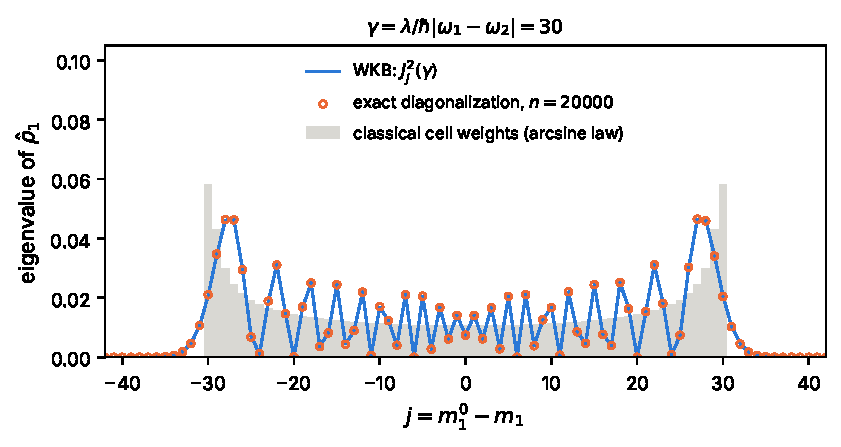
\includegraphics[width=0.8\textwidth]{fig1_weights.pdf}
\caption{Eigenvalues of the reduced density matrix of one branch of a highly excited
eigenstate, $J_{j}^{2}(\gamma)=2\Lambda_{j}$, at $\gamma=30$ (blue line), compared
with exact diagonalization of the sector Hamiltonian at $n=20\,000$,
$\lambda I/\hbar^{2}=6\times10^{5}$ (circles), and with the classical distribution
\eqref{eq:w} integrated over unit cells (grey bars). The quantum eigenvalues
oscillate with full contrast about the classical ones.}
\label{fig:weights}
\end{figure}

\subsection{Entanglement entropy}

The entanglement entropy is
\begin{equation}
S_{E}=-2\sum_{j}\Lambda_{j}\ln\Lambda_{j}
=\ln2-\sum_{j}J_{j}^{2}(\gamma)\ln J_{j}^{2}(\gamma).
\label{eq:SE1}
\end{equation}
For $\gamma\gg1$ we insert Eq.~\eqref{eq:Debye}. If the fringes are averaged away,
$J_{j}^{2}\to w(j)$, the sum becomes the integral
$-\int\dd j\,w\ln w=\ln(\pi\gamma/2)$ and $S_{E}\to\ln(\pi\gamma)$, which is
$S_{CE}$ with $\Delta=h$. The fringes, however, cannot be averaged away inside the
logarithm. Writing
$-J_{j}^{2}\ln J_{j}^{2}=-w(1+\cos\Phi_{j})[\ln w+\ln(1+\cos\Phi_{j})]$, the term
$w\cos\Phi_{j}\ln w$ averages to zero because $\Phi_{j}$ varies on the scale of a
cell while $w$ varies on the scale of $\gamma$. In the remaining term the phases
$\Phi_{j}$ are uniformly distributed, and (Appendix~\ref{app:asym})
\begin{equation}
\frac{1}{2\pi}\int_{0}^{2\pi}\dd\Phi\,(1+\cos\Phi)\ln(1+\cos\Phi)=1-\ln2 .
\label{eq:phaseavg}
\end{equation}
Hence
\begin{equation}
\boxed{\;S_{E}=\ln(\pi\gamma)-(1-\ln2)=\ln\frac{2\pi\gamma}{e}
=\ln\left[\frac{2\pi}{e}\,\frac{\lambda}{\hbar|\omega_{1}-\omega_{2}|}\right]\;}
\label{eq:SE}
\end{equation}
up to corrections that vanish as $\gamma\to\infty$. Numerically, the sum in
Eq.~\eqref{eq:SE1} approaches Eq.~\eqref{eq:SE} as $0.965\,\gamma^{-1/3}$; we have
checked this up to $\gamma=10^{6}$ (Fig.~\ref{fig:entropy} and
Appendix~\ref{app:num}). The $\gamma^{-1/3}$ comes from the edges of the band, where
the fringes become slow and the phase average fails.

Comparing Eqs.~\eqref{eq:SE} and \eqref{eq:SCE}, the classical and quantum
entanglement entropies have the same dependence on the coupling and on the
energies; the leading logarithm, $\ln[\lambda/\hbar|\omega_{1}-\omega_{2}|]$, is
identical. They are exactly equal if the elementary phase-space cell is chosen as
\begin{equation}
\Delta=\frac{e\,h}{2}=\pi e\,\hbar ,
\label{eq:Delta}
\end{equation}
to be compared with $\Delta=h/2$ for the oscillators of Ref.~\cite{DKS}. With the cell
$\Delta=h$ suggested by the quantization of angular momentum, the classical entropy
is larger than the quantum one by the universal constant
\begin{equation}
S_{CE}\big|_{\Delta=h}-S_{E}=1-\ln2\simeq0.307 .
\label{eq:deficit}
\end{equation}
This constant depends neither on $\lambda$ nor on the energies.

\begin{figure}[t]
\centering
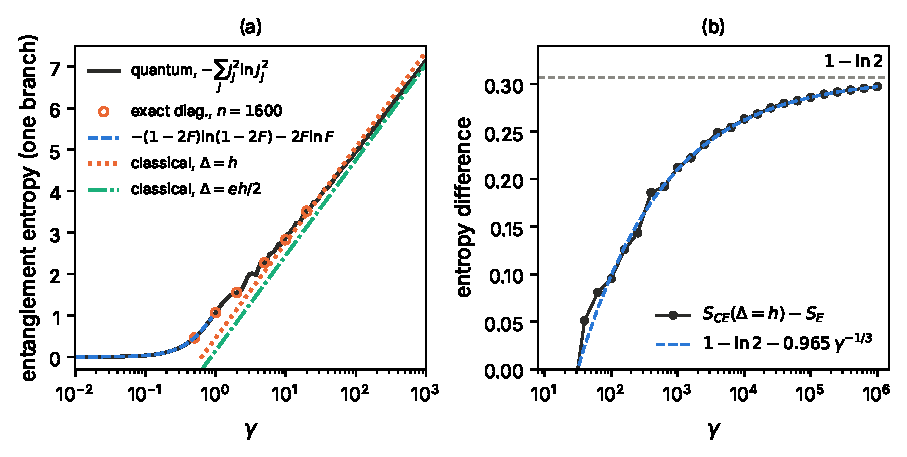
\includegraphics[width=\textwidth]{fig2_entropy.pdf}
\caption{(a) Entanglement entropy of one branch (the full eigenstate adds $\ln2$ to
every curve) as a function of $\gamma=\lambda/\hbar|\omega_{1}-\omega_{2}|$. Solid:
$-\sum_{j}J_{j}^{2}\ln J_{j}^{2}$, Eq.~\eqref{eq:SE1}; circles: exact diagonalization at
$n=1600$; dashed: the quantum-regime result \eqref{eq:SEn} with $F=\gamma^{2}/4$;
dotted: the classical entropy \eqref{eq:SCE} with $\Delta=h$; dash-dotted: with
$\Delta=eh/2$. (b) Difference between the classical ($\Delta=h$) and quantum
entropies, approaching $1-\ln2$ as $\gamma^{-1/3}$.}
\label{fig:entropy}
\end{figure}

The origin of the difference from the oscillator case is instructive. In
Ref.~\cite{DKS} the two classical branches compatible with one value of the observed
coordinate, $\sin[(S_{n+\delta n}(x))/\hbar]$ and $\sin[(S_{n-\delta n}(x))/\hbar]$,
can be recombined into two orthonormal eigenfunctions $\phi^{1,2}_{\delta n}$ of the
reduced density matrix. Their interference is then carried by the eigenvectors, and
the eigenvalues follow the smooth classical law. For the rotors, conservation of
total angular momentum fixes the eigenvectors of the reduced density matrix to be
angular-momentum eigenstates, so the interference between the two branches
$\varphi=\pm\arccos\xi$ cannot be absorbed into them. It appears in the eigenvalues
instead, as the fringes of Eq.~\eqref{eq:Debye}, and lowers the entropy by the phase
average \eqref{eq:phaseavg}.

The ingredients of the comparison are the same in both calculations. For a state of
one branch only --- a single sense of relative rotation, which is stationary on time
scales short compared with the inverse doublet splitting --- the same calculation
gives $\Lambda_{j}=J_{j}^{2}(\gamma)$ without degeneracy, and both $S_{E}$ and
$S_{CE}$ are lower by $\ln2$.

%=============================================================================
\section{Discussion}
\label{sec:disc}
%=============================================================================

We have computed the classical entanglement entropy of two weakly coupled rotors,
Eq.~\eqref{eq:SCE}, and the von Neumann entropy of a highly excited eigenstate in the
regime where the interaction energy is large on the quantum scale,
Eq.~\eqref{eq:SE}. As for the oscillators of Ref.~\cite{DKS}, the two have the same
leading logarithm. The exact equality is again contingent on the choice of the
phase-space cell, here $\Delta=eh/2$. Unlike the oscillators, the rotors suggest a
cell of their own, $\Delta=h$, and with it the two entropies differ by $1-\ln2$.

The reduced density matrix \eqref{eq:rho} describes a mixture of states with angular
momenta between $m_{1}^{0}-\gamma$ and $m_{1}^{0}+\gamma$ (and the mirror set), with
probabilities whose average is the classical distribution and vanishes outside this
range. In this sense it is close to a maximally entangled state, as in the
oscillator case, and its leading entropy has a classical origin. The probabilities
themselves, however, oscillate between zero and twice the classical value, and the
constant term of the entropy carries this quantum interference.

It is interesting to compare with the ground state. The perturbative calculation of
Appendix~\ref{app:pt} gives the reduced density matrix of an arbitrary eigenstate
that reduces to $\ket{m_{1},m_{2}}$ at $\lambda=0$. For the ground state,
$m_{1}=m_{2}=0$, it is
\begin{equation}
\hat\rho_{1}=(1-2f)\ketbra00+f\left(\ketbra11+\ketbra{-1}{-1}\right),\qquad
f=\left(\frac{\lambda I}{2\hbar^{2}}\right)^{2},
\label{eq:rho0}
\end{equation}
so that
\begin{equation}
S^{0}_{E}=-(1-2f)\ln(1-2f)-2f\ln f .
\label{eq:S0}
\end{equation}
The factor $f$ is the square of the ratio of the matrix element $\lambda/2$ to the
level spacing $\hbar^{2}/I$. The structure is that of the oscillator ground state,
$S^{0}_{E}=-(1-f)\ln(1-f)-f\ln f$ of Ref.~\cite{DKS}, except that the cosine
coupling transfers angular momentum in both directions, so that two states rather
than one are admixed. The term $-(1-2f)\ln(1-2f)\simeq2f$ comes entirely from the
$O(\lambda^{2})$ normalization of the perturbed state, which multiplies the
unperturbed component: without it $\Tr\hat\rho_{1}=1+2f$, and the entropy would be
low by a fraction $1/[1+\ln(1/f)]$, which vanishes only logarithmically as
$\lambda\to0$ (Appendix~\ref{app:pt}).

A similar result holds for a highly excited state in the quantum regime, where the
energy of the relative motion is large but the interaction energy is small on the
quantum scale, $\gamma\ll1$. Expanding the WKB wave function \eqref{eq:uexp} to
second order in $\gamma$,
\begin{equation}
e^{-i\gamma\sin\varphi}\simeq\left(1-\frac{\gamma^{2}}{4}\right)
-\frac{\gamma}{2}\,e^{i\varphi}+\frac{\gamma}{2}\,e^{-i\varphi}
+\frac{\gamma^{2}}{8}\left(e^{2i\varphi}+e^{-2i\varphi}\right),
\label{eq:smallgamma}
\end{equation}
the branch $m_{1}^{0}$ has reduced density matrix
\begin{equation}
\begin{gathered}
\hat\rho_{1}=(1-2F)\ketbra{m_{1}^{0}}{m_{1}^{0}}
+F\left(\ketbra{m_{1}^{0}+1}{m_{1}^{0}+1}+\ketbra{m_{1}^{0}-1}{m_{1}^{0}-1}\right),\\
F=\frac{\gamma^{2}}{4}=\left(\frac{\lambda}{2\hbar|\omega_{1}-\omega_{2}|}\right)^{2},
\end{gathered}
\label{eq:rhon}
\end{equation}
to order $\gamma^{2}$, and
\begin{equation}
S^{n}_{E}=-(1-2F)\ln(1-2F)-2F\ln F
\label{eq:SEn}
\end{equation}
(plus $\ln2$ for the parity eigenstate). The depletion $1-2F$ of the central weight
again comes from the second-order term of the unperturbed amplitude,
$1-\gamma^{2}/4$. Equation~\eqref{eq:rhon} coincides with the large-$|n|$ limit of
the perturbative result of Appendix~\ref{app:pt}, $\varepsilon_{\pm}=\alpha^{2}/(n\pm1)^{2}
\to\gamma^{2}/4$. For $F\ll1$ the result is thus identical in form to the ground
state, as in the oscillator case.

The same parameter controls the classical regime. With $\gamma=2F^{1/2}$,
Eqs.~\eqref{eq:SCE} and \eqref{eq:SE} read
\begin{equation}
S_{CE}\big|_{\Delta=h}=\ln\left(2\pi F^{1/2}\right),\qquad
S_{E}=\ln\left(\frac{4\pi}{e}F^{1/2}\right)\qquad(F\gg1).
\label{eq:Sclassreg}
\end{equation}
As for the oscillators, the result \eqref{eq:SEn} holds for $F\ll1$ and the classical
result for $F\gg1$. In the classical regime the reduced density matrix is a mixture
of $\sim F^{1/2}$ states with small probabilities, and the entropy is
$S\approx\ln F^{1/2}$. The crossover between the two regimes is smooth
[Fig.~\ref{fig:entropy}(a)]: the Bessel form \eqref{eq:SE1} interpolates between
Eq.~\eqref{eq:SEn} at $\gamma\ll1$ and Eq.~\eqref{eq:SE} at $\gamma\gg1$.

These results parallel the discussion in Refs.~\cite{DKS,KharzeevLevin}. If $F$ is
identified with the parton density, the perturbative regime $F\ll1$ reproduces the
form of the entropy posited in Ref.~\cite{KharzeevLevin}, and the classical regime,
in which the coupling is weak but the number of excitations is large, $F\gg1$, gives
an entropy $\ln F^{1/2}$ with the same additional power $1/2$ under the logarithm
found for the oscillators. The rotor model shows, however, that the constant term
need not be classical: when a conservation law ties the Schmidt basis to the
observed degree of freedom, the interference between classical branches survives in
the entanglement spectrum, and the entropy falls below its classical value by a
universal amount. Whether such constants survive in chaotic systems with many
degrees of freedom, which are closer to the quasi-thermal states of high-energy
collisions, is an interesting open question.

\begin{acknowledgments}
[To be completed.]
\end{acknowledgments}

\appendix

%=============================================================================
\section{Perturbation theory and the density matrix to second order}
\label{app:pt}
%=============================================================================

We expand about the unperturbed state $\ket{m_{1},m_{2}}$ in sector $M$, with
relative quantum number $n=m_{1}-m_{2}$, writing
\begin{equation}
\ket{\Psi}=\mathcal{N}\left[\ket{m_{1},m_{2}}+\lambda\ket{\psi^{(1)}}
+\lambda^{2}\ket{\psi^{(2)}}\right]+O(\lambda^{3}),\qquad
E=E^{(0)}_{m_{1},m_{2}}+\lambda E^{(1)}+\lambda^{2}E^{(2)}+O(\lambda^{3}),
\label{eq:ptexp}
\end{equation}
with $\braket{m_{1},m_{2}}{\psi^{(k)}}=0$. By Eq.~\eqref{eq:V} the diagonal matrix
element of the coupling vanishes, so $E^{(1)}=0$, and the only states connected to
$\ket{m_{1},m_{2}}$ are $\ket{m_{1}\pm1,m_{2}\mp1}$, with matrix element $1/2$ and
energy denominators
\begin{equation}
E^{(0)}_{m_{1},m_{2}}-E^{(0)}_{m_{1}\pm1,m_{2}\mp1}
=\frac{\hbar^{2}}{2I}\left[\mp2m_{1}\pm2m_{2}-2\right]=\mp\frac{\hbar^{2}}{I}(n\pm1).
\label{eq:denoms}
\end{equation}
With $\alpha=\lambda I/2\hbar^{2}$, non-degenerate perturbation theory gives, for
$n\neq\pm1,\pm2$,
\begin{align}
\lambda\ket{\psi^{(1)}}&=-\frac{\alpha}{n+1}\ket{m_{1}+1,m_{2}-1}
+\frac{\alpha}{n-1}\ket{m_{1}-1,m_{2}+1},\label{eq:psi1}\\
\lambda^{2}\ket{\psi^{(2)}}&=\frac{\alpha^{2}}{2(n+1)(n+2)}\ket{m_{1}+2,m_{2}-2}
+\frac{\alpha^{2}}{2(n-1)(n-2)}\ket{m_{1}-2,m_{2}+2},\label{eq:psi2}\\
E^{(2)}\lambda^{2}&=\frac{\lambda^{2}I}{2\hbar^{2}(n^{2}-1)} .\label{eq:E2}
\end{align}
At $n=\pm1$ the states $n$ and $-n$ are degenerate and connected at first order, and
at $n=\pm2$ at second order; these cases require degenerate perturbation theory.

\emph{Normalization.} Since $\ket{\psi^{(1)}}$ and $\ket{\psi^{(2)}}$ are orthogonal to
$\ket{m_{1},m_{2}}$,
$\braket{\Psi}{\Psi}=\mathcal{N}^{2}[1+\epsp+\epsm]+O(\lambda^{4})$, with
\begin{equation}
\varepsilon_{\pm}=\frac{\alpha^{2}}{(n\pm1)^{2}}=\frac{\lambda^{2}I^{2}}{4\hbar^{4}(n\pm1)^{2}},
\qquad
\mathcal{N}=1-\frac{\lambda^{2}I^{2}}{8\hbar^{4}}\left[\frac{1}{(n+1)^{2}}
+\frac{1}{(n-1)^{2}}\right]+O(\lambda^{4}).
\label{eq:norm}
\end{equation}
In the state, $\mathcal{N}-1$ is of second order, beyond the accuracy to which the
admixed amplitudes are kept, and it can be dropped. In the density matrix it cannot:
$\rho$ is bilinear in the amplitudes, and the coefficient of
$\ketbra{m_{1},m_{2}}{m_{1},m_{2}}$ is $\mathcal{N}^{2}=1-\epsp-\epsm$, a correction of
the same order as the populations $\varepsilon_{\pm}$.

\emph{Density matrix.} To second order,
\begingroup\small
\begin{align}
\rho={}&\ketbra{m_{1},m_{2}}{m_{1},m_{2}}\nonumber\\
&-\frac{\lambda I}{2\hbar^{2}(n+1)}\Big[\ketbra{m_{1}+1,m_{2}-1}{m_{1},m_{2}}
+\ketbra{m_{1},m_{2}}{m_{1}+1,m_{2}-1}\Big]\nonumber\\
&+\frac{\lambda I}{2\hbar^{2}(n-1)}\Big[\ketbra{m_{1}-1,m_{2}+1}{m_{1},m_{2}}
+\ketbra{m_{1},m_{2}}{m_{1}-1,m_{2}+1}\Big]\nonumber\\
&+\frac{\lambda^{2}I^{2}}{4\hbar^{4}(n+1)^{2}}\ketbra{m_{1}+1,m_{2}-1}{m_{1}+1,m_{2}-1}
\nonumber\\
&+\frac{\lambda^{2}I^{2}}{4\hbar^{4}(n-1)^{2}}\ketbra{m_{1}-1,m_{2}+1}{m_{1}-1,m_{2}+1}
\nonumber\\
&-\frac{\lambda^{2}I^{2}}{4\hbar^{4}(n-1)(n+1)}\Big[\ketbra{m_{1}-1,m_{2}+1}{m_{1}+1,m_{2}-1}
+\ketbra{m_{1}+1,m_{2}-1}{m_{1}-1,m_{2}+1}\Big]\nonumber\\
&+\frac{\lambda^{2}I^{2}}{8\hbar^{4}(n+1)(n+2)}\Big[\ketbra{m_{1}+2,m_{2}-2}{m_{1},m_{2}}
+\ketbra{m_{1},m_{2}}{m_{1}+2,m_{2}-2}\Big]\nonumber\\
&+\frac{\lambda^{2}I^{2}}{8\hbar^{4}(n-1)(n-2)}\Big[\ketbra{m_{1}-2,m_{2}+2}{m_{1},m_{2}}
+\ketbra{m_{1},m_{2}}{m_{1}-2,m_{2}+2}\Big]\nonumber\\
&-\frac{\lambda^{2}I^{2}}{4\hbar^{4}}\left[\frac{1}{(n+1)^{2}}+\frac{1}{(n-1)^{2}}\right]
\ketbra{m_{1},m_{2}}{m_{1},m_{2}}+O(\lambda^{3}).
\label{eq:rhofull}
\end{align}
\endgroup
The last line is the normalization term. Its coefficient is
$\epsp+\epsm$, twice the coefficient $\lambda^{2}I^{2}[\dots]/8\hbar^{4}$ that
$\ket{m_{1},m_{2}}$ carries in the state, because $\mathcal{N}$ multiplies both the ket
and the bra. With this coefficient $\Tr\rho=(1-\epsp-\epsm)+\epsp+\epsm=1$ and
$\Tr\rho^{2}=(1-\epsp-\epsm)^{2}+2(\epsp+\epsm)+O(\lambda^{4})=1$; with the
coefficient halved, both fail at order $\lambda^{2}$.

\emph{Reduced density matrix.} Using $\Tr_{2}\ketbra{a,b}{c,d}=\delta_{bd}\ketbra ac$,
every off-diagonal term of Eq.~\eqref{eq:rhofull} connects different values of $m_{2}$
and drops out, including the second-order amplitudes. This is a consequence of the
conservation of $M$: each value of $m_{1}$ is paired with a single value of $m_{2}$.
The result is
\begin{equation}
\hat\rho_{1}=\left(1-\epsp-\epsm\right)\ketbra{m_{1}}{m_{1}}
+\epsp\ketbra{m_{1}+1}{m_{1}+1}+\epsm\ketbra{m_{1}-1}{m_{1}-1}+O(\lambda^{4}),
\label{eq:rho1pt}
\end{equation}
the error being $O(\lambda^{4})$ because the $O(\lambda^{3})$ terms of $\rho$ are all
off-diagonal in $m_{2}$. The entanglement and linear entropies are
\begin{equation}
S_{E}=\epsp\ln\frac{1}{\epsp}+\epsm\ln\frac{1}{\epsm}+\left(\epsp+\epsm\right)
+O(\varepsilon^{2}),\qquad
S_{L}=1-\Tr\hat\rho_{1}^{2}=2\left(\epsp+\epsm\right)+O(\varepsilon^{2}).
\label{eq:Spt}
\end{equation}
The non-logarithmic term of $S_{E}$ and the whole of $S_{L}$ come from the
normalization term. For $n=0$ (which includes the ground state) $\varepsilon_{\pm}=
\alpha^{2}=f$, which gives Eq.~\eqref{eq:rho0}. For $|n|\gg1$,
$\varepsilon_{\pm}\to\alpha^{2}/n^{2}=\gamma^{2}/4=F$, which gives Eq.~\eqref{eq:rhon}.
For the exact eigenstates, which are even or odd under exchange, the entropy is larger
by $\ln2$ when $|n|\ge3$, since the two exchange partners then overlap only at order
$\lambda^{|n|}$.

%=============================================================================
\section{Asymptotic evaluation of the quantum entropy}
\label{app:asym}
%=============================================================================

\emph{The phase average.} With $1+\cos\Phi=2\cos^{2}(\Phi/2)$ and Eq.~\eqref{eq:GR},
$\frac{1}{2\pi}\int_{0}^{2\pi}\ln(1+\cos\Phi)\,\dd\Phi=\ln2+\frac{2}{\pi}\int_{0}^{\pi}
\ln|\cos t|\,\dd t=-\ln2$. Integrating by parts,
$\frac{1}{2\pi}\int_{0}^{2\pi}\cos\Phi\ln(1+\cos\Phi)\,\dd\Phi=\frac{1}{2\pi}\int_{0}^{2\pi}
\frac{\sin^{2}\Phi}{1+\cos\Phi}\dd\Phi=\frac{1}{2\pi}\int_{0}^{2\pi}(1-\cos\Phi)\dd\Phi=1$.
The sum is Eq.~\eqref{eq:phaseavg}.

\emph{The classical part.} With $j=\gamma\cos\beta$, $w(j)\,\dd j=\dd\beta/\pi$ and
$-\int w\ln w\,\dd j=\ln\pi+\frac1\pi\int_{0}^{\pi}\ln(\gamma\sin\beta)\dd\beta=\ln(\pi\gamma/2)$.

\emph{The fringes.} The local wavenumber of the fringes is
$\dd\Phi_{j}/\dd j=-2\arccos(j/\gamma)\in(-2\pi,0)$, so $\Phi_{j}$ modulo $2\pi$ is
equidistributed over the band except near its edges, $|j|\to\gamma$, where the
wavenumber tends to $0$ or $2\pi$ and the fringes become stationary. Near
$j=\gamma-\delta$ the phase accumulated over the last $\delta$ cells is
$\simeq\frac{4\sqrt2}{3}\delta^{3/2}/\sqrt\gamma$, which reaches $2\pi$ at
$\delta\sim\gamma^{1/3}$, and the classical weight within that distance of the edges is
$\sim\gamma^{-1/3}$. Hence $-\sum_{j}J_{j}^{2}\ln J_{j}^{2}=\ln(\pi\gamma/2)-(1-\ln2)
+O(\gamma^{-1/3})$; numerically the coefficient of $\gamma^{-1/3}$ is $0.965$.

%=============================================================================
\section{Numerical checks}
\label{app:num}
%=============================================================================

All checks use $\hbar=I=1$. Exact eigenstates are obtained by diagonalizing the sector
Hamiltonian $h_{kk'}=k^{2}\delta_{kk'}+\frac{\lambda}{2}(\delta_{k',k+1}+\delta_{k',k-1})$
in a window of $k$ around $k_{0}=n/2$ wide enough to contain the band. The classical
trajectory is integrated from Eq.~\eqref{eq:eom} with
$\lambda=400$, $\Erel=2500$, $J=0$ (so $a=4$) over $t=2000$, and the time spent by
$p_{1}$ in each unit cell is compared with the integral of Eq.~\eqref{eq:Wexact}.
Table~\ref{tab:checks} lists the results.

\begin{table}[h]
\caption{Analytic results against numerics ($\hbar=I=1$).}
\label{tab:checks}
\begin{ruledtabular}
\begin{tabular}{lll}
quantity & analytic & numerical\\
\hline
eigenvalues at $n=20000$, $\gamma=30$: $\max_{j}|p_{j}-J_{j}^{2}|$ & 0 & $4.1\times10^{-4}$\\
entropy at $n=20000$, $\gamma=30$, Eq.~\eqref{eq:SE1} (one branch) & 3.858110 & 3.858114\\
entropy at $n=20000$, $\gamma=5$ (one branch) & 2.271422 & 2.271422\\
$p_{j=0}$ at $n=800$, $\gamma=5$, vs $J_{0}^{2}(5)$ & 0.0315406 & 0.0315284\\
$-\sum J_{j}^{2}\ln J_{j}^{2}$ at $\gamma=0.02$ vs Eq.~\eqref{eq:SEn} & $2.04205\times10^{-3}$ & $2.04197\times10^{-3}$\\
$-\sum J_{j}^{2}\ln J_{j}^{2}-\ln(\pi\gamma/e)$ at $\gamma=10^{6}$ & $0.965\gamma^{-1/3}=0.00965$ & 0.00966\\
$\ln(\pi\gamma/2)+\sum J_{j}^{2}\ln J_{j}^{2}$ at $\gamma=10^{6}$ vs $1-\ln2$ & 0.306853 & 0.297194\\
classical trajectory: cell weights vs Eq.~\eqref{eq:Wexact} & 0 & $3.7\times10^{-6}$\\
classical entropy of one band ($\Delta=h$), exact vs Eq.~\eqref{eq:SCE} & 1.84029 & 1.83788\\
$p_{0}=1-\epsp-\epsm$, $(m_{1},m_{2})=(4,4)$, $\lambda=0.02$ & 0.99980000 & 0.99980011\\
$S_{E}$, $(m_{1},m_{2})=(4,4)$, $\lambda=0.02$, Eq.~\eqref{eq:Spt} & $2.04207\times10^{-3}$ & $2.04106\times10^{-3}$\\
same without the normalization term & $1.84207\times10^{-3}$ & \\
$S_{E}$, $(m_{1},m_{2})=(9,2)$, $\lambda=0.2$, Eq.~\eqref{eq:Spt} & $4.07805\times10^{-3}$ & $4.07776\times10^{-3}$\\
\end{tabular}
\end{ruledtabular}
\end{table}

\begin{thebibliography}{99}

\bibitem{Klco} N.~Klco, A.~Roggero, and M.~J.~Savage, arXiv:2107.04769.
\bibitem{KharzeevLevin} D.~E.~Kharzeev and E.~M.~Levin, Phys.\ Rev.\ D \textbf{95},
114008 (2017).
\bibitem{Hagiwara} Y.~Hagiwara, Y.~Hatta, B.-W.~Xiao, and F.~Yuan, Phys.\ Rev.\ D
\textbf{97}, 094029 (2018).
\bibitem{TuKharzeev} Z.~Tu, D.~E.~Kharzeev, and T.~Ullrich, Phys.\ Rev.\ Lett.\
\textbf{124}, 062001 (2020).
\bibitem{Baier} R.~Baier, A.~H.~Mueller, D.~Schiff, and D.~T.~Son, Phys.\ Lett.\ B
\textbf{502}, 51 (2001).
\bibitem{Berges} J.~Berges, M.~P.~Heller, A.~Mazeliauskas, and R.~Venugopalan,
Rev.\ Mod.\ Phys.\ \textbf{93}, 035003 (2021).
\bibitem{Deutsch} J.~M.~Deutsch, Rep.\ Prog.\ Phys.\ \textbf{81}, 082001 (2018).
\bibitem{DKS} H.~Duan, A.~Kovner, and V.~V.~Skokov, Classical entanglement and
entropy, arXiv:2301.05735.
\bibitem{GR} I.~S.~Gradshteyn and I.~M.~Ryzhik, \emph{Table of Integrals, Series, and
Products}, 7th ed.\ (Academic, New York, 2007).
\bibitem{DLMF} NIST Digital Library of Mathematical Functions, \S10.12 (generating
function and Jacobi--Anger expansion) and \S10.19(ii) (Debye expansions),
\url{https://dlmf.nist.gov/10}.

\end{thebibliography}

\end{document}
